% !TEX root = ../main.tex

% = = = = = = = = = = = = = = = = = = = %
%             Introduction              % 
% = = = = = = = = = = = = = = = = = = = %

\let\clearpage\relax
\chapter{Introduction}

During the past decade, people have tried to build machines with better computing performance. Frequency scaling was first used to enhance the performance of the system. Since clock frequency is the ``heart rate'' of a computer, frequency ramping has traditionally been the dominant force in the improvement of performance for commodity processors from the mid-1980s to about the end of 2004 \cite{frequency_ramping}.  However, increases in frequency also lead to increases in power consumption.  It was also because of the power wall that Intel canceled its Tejas and Jayhawk processors in 2004 \cite{intel}.

Fig.~\ref{frequency} illustrates the improvement in clock frequency over time, measured in megahertz (millions of cycles per second). Clearly, clock-frequency improvements have been stalled and limited to about 3-4GHz due to power consumption nowadays \cite{nap}.
\begin{figure}[!htp]
    \centering
    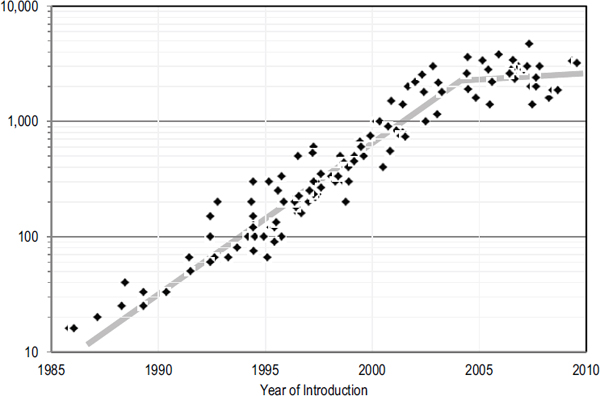
\includegraphics[width=0.8\linewidth]{figure/frequency.jpg}
    \caption{Microprocessor clock frequency (MHz) over time (1985-2010) \cite{nap}.}
    \label{frequency}
\end{figure}

In order to continuously improve the computing performance without depending on Moore's Law, people use parallel computing instead of sequential computing nowadays. What's more, products with parallel hardware and chip multi-processors has become one of the mainstream in the microprocessor industry \cite{nap}.

In addition to the parallel computing, people also leave the optimization of computer architecture as the future of computing. Domain-specific architecture design and optimization is one of these topics and it is really hot these days because of the need for AI and other applications. A groundbreaking example for domain-specific architecture is Google's tensor processing unit (TPU), which was first deployed in 2015 and now serves more than 1 billion people. Compared with contemporary CPUs and GPUs using similar technologies, it runs deep neural networks (DNN) 15 to 30 times faster and has 30 to 80 times better energy efficiency \cite{xxx}.

The biggest challenge in domain-specific architecture design was raised from the domain of the embedded system. These days embedded system start to adapt algorithms which need very large computing power. For example, Tesla's automotive car needs to process millions of pixels in short latency and feed them to the AI algorithm \cite{Tesla}.

Traditional AI computing platform like a CPU cannot provide so much computing power. Not only the computation limits the design, but energy efficiency is also vital for some system. A smart camera usually can be supplied limited1 energy. A camera on the drone, for example, must save energy to enlarge battery life. However, smart embedded systems do need complicated operations to implement neural networks, which usually costs lots of energy which is a dilemma. Finally, embedded systems are limited by cost. Generally, the engine controller under the hood of the car and the chip in the mobile phone needs to be below \$3-5 \cite{nap}. The chip in tennis shoes or greeting cards is even cheaper and cannot have a large chip area. Due to these reasons, some techniques like Single instruction, multiple threads (SIMT) may not be appropriate for such kind of system. Therefore, the need for an embedded system really calls for a novel design in computer architecture that can balance performance, energy efficiency, and cost for computation-intensive tasks.

There are some recent achievements in improving computer performance through optimizing of computer architecture. In a study applied in an application specific integrated circuit design (ASIC design), an high-accuracy approximate adder is introduced which can decrease the power and delay with a low relative error\cite{paper1}. Subsequently, a study introduces approximate operators into DNN hardware accelerators to reduce latency and energy consumption \cite{paper2}. Another study applies approximate divider and square root operations on their RISC-V design \cite{paper3}. But all these studies narrow their designs in some specific fields and the approximate adders and approximate operators actually can be used in a wide range of computing components including CPU, GPU and SoC. In this project, we propose an out-of-order processor design based on RISC-V with approximate computing units to reach a general solution for SoC design that can balance performance, energy and cost.

In this report, a short introduction and related works will be given in chapter 1 and 2. We will discuss our customer requirements and engineering specifications in chapter 3. Then the process of concept generation and selection will be discussed in details in chapter 4 and 5, followed by our final design of microarchitecture design and optimization in chapter 6. Implementation and validation will be discussed in chapter 7. Finally, our discussion, future work and conclusion of this project will be in chapter 8 and 9.
